\documentclass[a4paper, titlepage]{livret} % classe spéciale rapport : livret

\usepackage[utf8]{inputenc} % accents
\usepackage[T1]{fontenc} % caractères français
\usepackage{geometry} % marges
\usepackage[francais]{babel} % langue
\usepackage{graphicx} % images
\usepackage{verbatim} % texte préformaté
\usepackage{listings} % code source
\usepackage[framed,numbered,autolinebreaks,useliterate]{mcode} % code source
\usepackage{listingsutf8} % code source accents
\usepackage[final]{pdfpages} % inclusion de pdf
\usepackage{url} % utilisation des url
\usepackage{caption} % caption pour les figures
\usepackage{amsmath} % maths
\usepackage{amsfonts, bbm} % fonts maths

\def\siecle#1{\textsc{\romannumeral #1}\textsuperscript{e}} % macro pour l'écriture des siècles
\graphicspath{{img/}} % chemin des illustrations
\lstset{language=C,
	inputencoding=utf8/latin1
} % langage C

\title{TP d'Algorithmique Numérique} % titre
\author{Elliot Sisteron} % auteur

\pagestyle{headings} % rappel discret du titre en cours (en haut à gauche)

\begin{document} % début du document

	
\includepdf{pdf/cover.pdf} % page de garde
	
	\chapter*{Introduction}
	\addcontentsline{toc}{chapter}{Introduction} % ajouter l'introduction au sommaire
		Depuis la création des \og bombes \fg{} destinées à déchiffrer des messages codés pendant la seconde guerre mondiale, les appareils informatiques ont connu un essor exponentiel.
		Non seulement l'informatique est aujourd'hui omniprésente, mais elle continue d'évoluer de jour en jour (les conjectures de Moore évaluent que la puissance brute des machines doublerai tout les deux ans).
		D'abord pensés pour réaliser des calculs, il est logique de vouloir que nos ordinateurs manient des objets aussi abstraits que les nombres réels.
		Or, il est difficile de gérer des nombres à virgules en binaire, d'où la nécessité d'imposer une norme de codage de ces nombres (on pense notamment aux incidents de la bourse de Vancouver, du missile Patriote ou encore de la fusée Arianne).
		C'est la raison pour laquelle on a vu apparaître ces dernières années la norme \emph{IEEE 754} destinée à régulariser la représentation des nombres à virgule flottante en binaire.

		Cette convention consiste à représenter en machine les nombres à virgules flottantes (ou \og flottants \fg) de la manière suivante : $(-1)^s \times (1+m) \times 2^{(e - d)}$.\\
		Avec :
		\begin{itemize}
			\item un nombre $s$ sur un bit pour déterminer le signe ($1$ pour négatif, $0$ pour positif);
			\item $m$ pour la valeur décimale de la \og mantisse \fg{} : la partie fractionnaire en notation binaire scientifique. La mantisse tient sur plusieurs bits; la convention est de 23 bits pour un stockage du nombre sur 32 bits (respectivement 52 pour 64);
			\item $e$ pour l'exposant signé de la puissance de $2$, codé sur 8 bits en simple précision (respectivement 11 en double);
			\item $d$ pour le décalage de l'exposant afin de le stocker sous forme d'un nombre non-signé (codage de l'exposant par excès). Si l'on note $b$ le nombre de bits codant l'exposant, on a $d = 2^{b-1}-1$.
		\end{itemize}
		Dans ce cas, on dira que le nombre flottant est \og normalisé \fg{}.
		Pour un nombre très proche de $0$ (i.e. dont l'exposant dépasse la capacité du format), on qualifiera le flottant de \og dénormalisé \fg{} et on prendra une représentation légèrement différente pour pouvoir le coder : $(-1)^s \times m \times 2^{(1 -d)}$ (l'exposant est représenté comme étant minimal mais sa valeur est $1 - d$ pour assurer une sorte de continuité entre le zéro, les nombres dénormalisés et les nombres normalisés). Le premier bit de la mantisse qui est implicitement $1$ en normalisé est ici, de manière implicite aussi, $0$.

		Dans ce TP, on se propose d'étudier différents flottants; tant bien en s'intéressant à leurs représentations en binaire, mais aussi en étudiant leurs valeurs exactes et décimales.
		Nous nous attarderons, dans un premier temps, sur des flottants caractéristiques de la norme \emph{IEEE 754} : 
		\begin{itemize}
			\item l'$\epsilon_{machine}$;
			\item $X_{min}$ normalisé/dénormalisé;
			\item $X_{max}$ normalisé/dénormalisé;
			\item le zéro : $0$ et l'unité : $1$.
		\end{itemize}	
		Puis, nous prendrons un autre exemple plus concret : nous nous intéresserons au codage de $0.1$.
		Ensuite, nous regarderons comment est codé une somme de termes inférieurs à l'$\epsilon_{machine}$.
		Enfin, nous étudierons le codage de l'unité ajouté à cette somme.

	\setcounter{tocdepth}{1} % profondeur table des matières
	\tableofcontents % table des matières
	
	\chapter{Étude de flottants caractéristiques}
		Dans cette partie, on s'intéresse à des flottants particuliers. 
		Ils sont importants dans le sens où ils définissent les limites du calcul scientifique sur machine.

		\section{L'$\epsilon_{machine}$}
			L'$\epsilon_{machine}$ est le plus petit réel positif-machine tel que : 1 + $\epsilon_{machine}$ > 1 sur machine.
			On développe un petit programme C pour pouvoir l'approximer, à un ordre de magnitude près :
			\lstinputlisting{"../Programmes/Epsilon machine/src/epsilonMachine.c"}

			Ce qui nous donne comme sortie à l'écran :
			\begin{figure}[!h]
				\centering
  					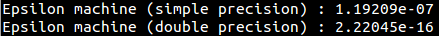
\includegraphics[scale=0.6]{Epsilon.png}
  					\caption{Résultat affiché par le programme}
			\end{figure}		

			On voudrait connaître la représentation binaire de ce flottant.
			Pour cela on passe par le débuggeur gdb (sans oublier de rajouter l'option -g en flag dans le makefile).
			On commence par poser un break sur la ligne où est affichée la variable que l'on souhaite étudier (ici, ligne $23$ pour la simple précision et $24$ pour la double précision), puis on lance le programme avec la commande \emph{run}.
			La commande \emph{x/tw} pour un simple, respectivement \emph{x/tg} pour un double, suivie de la valeur de l'adresse de cette variable (opérateur \&) nous permet de récupérer son codage en binaire.

			\subsection{Simple précision}
				\subsubsection{Codage binaire}
					En codage $32$ bits, on a :
					\begin{figure}[!h]
						\centering
  							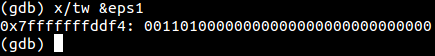
\includegraphics[scale=0.5]{BinaireEpsilonSimple.png}
  							\caption{Codage binaire de notre approximation de l'$\epsilon_{machine}$ en simple précision}
					\end{figure}

					On en déduit donc que le nombre flottant, en simple précision :
					\begin{itemize}
						\item est bien composé de $32$ bits;
						\item est positif (bit de signe à 0);
						\item est normalisé (l'exposant n'est pas codé par $00000000$);
						\item a un exposant dont le codage binaire est $01101000$;
						\item a une mantisse dont le codage binaire est $00000000 00000000 000000$.
					\end{itemize}

				\subsubsection{Valeur exacte}
					On a clairement : 
					\begin{itemize}
						\item le bit de signe $s = 0$;
						\item la valeur de la mantisse qui vaut $m = 0$.
					\end{itemize}
					Reste à trouver la valeur de l'exposant $e$, puis à le décaler de $d = 2^{8-1}-1 = 127$.
					On a l'expression binaire de l'exposant $(e)_{2} = (01101000)_{2} = (e_{7}e_{6}…e_{0})_{2}$.\\
					On en déduit la valeur en base $10$, 
					\[\begin{aligned}
						e & = \sum_{i=0}^{7} e_{i}2^{i}\\
						  & = 2^{3} + 2^{5} + 2^{6}\\
						  & = 8 + 32 + 64\\
						  & = 104
					\end{aligned}\]
					D'où $e-d = 104 - 127 = -23$.\\
					Finalement, la valeur $v$ du flottant binaire précédent est :
					\[\begin{aligned}
						v & = (-1)^{0} \times 1.0 \times 2^{-23}\\
						  & = 2^{-23}
					\end{aligned}\]

				\subsubsection{Valeur décimale}
					On en déduit la valeur décimale suivante :
					\[\begin{aligned}
						v & = 2^{-23}\\
						  & \approx 1.19 \times 10^{-7}
					\end{aligned}\]
					Ce qui confirme le résultat affiché à l'écran :
					\begin{figure}[!h]
						\centering
  							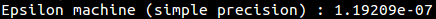
\includegraphics[scale=0.6]{EpsilonSimple.png}
  							\caption{Valeur décimale affichée de notre approximation de l'$\epsilon_{machine}$ simple}
					\end{figure}

			\subsection{Double précision}
				\subsubsection{Codage binaire}
					En codage $64$ bits, on a :
					\begin{figure}[!h]
						\centering
  							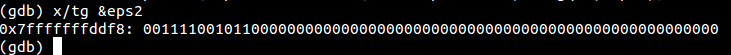
\includegraphics[scale=0.5]{BinaireEpsilonDouble.png}
  							\caption{Codage binaire de notre approximation de l'$\epsilon_{machine}$ en double précision}
					\end{figure}
	
					On en déduit donc que le nombre flottant, en double précision :
					\begin{itemize}
						\item est bien composé de $64$ bits;
						\item est positif (bit de signe à 0);
						\item est normalisé (l'exposant n'est pas codé par $00000000$);
						\item a un exposant dont le codage binaire est $01111001011$;
						\item a une mantisse dont le codage binaire est $00000000 00000000 0000000 0000000 00000000 00000000 0000$.
					\end{itemize}

				\subsubsection{Valeur exacte}
					On a clairement : 
					\begin{itemize}
						\item le bit de signe $s = 0$;
						\item la valeur de la mantisse qui vaut $m = 0$.
					\end{itemize}
					Reste à trouver la valeur de l'exposant $e$, puis à le décaler de $d = 2^{11-1}-1 = 1024$.
					On a l'expression binaire de l'exposant $(e)_{2} = (01111001011)_{2} = (e_{10}e_{9}…e_{0})_{2}$.\\
					On en déduit la valeur en base $10$, 
					\[\begin{aligned}
						e & = \sum_{i=0}^{10} e_{i}2^{i}\\
						  & = 2^{0} + 2^{1} + 2^{3} + 2^{6} + 2^{7} + 2^{8} + 2^{9}\\
						  & = 971
					\end{aligned}\]
					D'où $e-d = 971 - 1023 = -52$.\\
					Finalement, la valeur $v$ du flottant binaire précédent est :
					\[\begin{aligned}
						v & = (-1)^{0} \times 1.0 \times 2^{-52}\\
						  & = 2^{-52}
					\end{aligned}\]

				\subsubsection{Valeur décimale}
					On en déduit la valeur décimale suivante :
					\[\begin{aligned}
						v & = 2^{-52}\\
						  & \approx 2.22 \times 10^{-16}
					\end{aligned}\]
					Ce qui confirme le résultat affiché à l'écran :
					\begin{figure}[!h]
						\centering
  							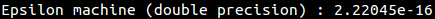
\includegraphics[scale=0.6]{EpsilonDouble.png}
  							\caption{Valeur décimale affichée de notre approximation de l'$\epsilon_{machine}$ double}
					\end{figure}

					En fait, les valeurs trouvées pour le $\epsilon_{machine}$ sont très logiques dans le sens où elle définissent la limite qu'impose la mantisse : après 23 bits en simple précision et 52 bits en double (respectivement $2^{-23}$ et $2^{-52}$ pour l'epsilon machine), on ne peut plus rien mettre dans la mantisse. 

		\section{$X_{min}$}
			$X_{min}$ est le plus petit nombre flottant que l'on peut coder sur machine.
			On développe un programme C pour pouvoir le calculer en normalisé et en dénormalisé :
			\lstinputlisting{"../Programmes/X min/src/xMin.c"}
			On va donc poser un break sur les lignes 45, 46, 47 et 48.

			Ce qui nous donne comme sortie à l'écran :
			\begin{figure}[!h]
				\centering
  					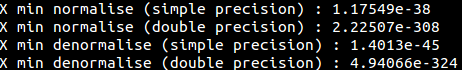
\includegraphics[scale=0.6]{XMin.png}
  					\caption{Résultat affiché par le programme}
			\end{figure}

			\subsection{$X_{min}$ normalisé en simple précision}
				\subsubsection{Codage binaire}
					En codage $32$ bits, on a :
					\begin{figure}[!h]
						\centering
  							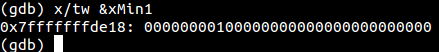
\includegraphics[scale=0.5]{BinaireXMinNormaliseSimple.png}
  							\caption{Codage binaire du $X_{min}$ normalisé en simple précision}
					\end{figure}

					On en déduit donc que le nombre flottant, en simple précision :
					\begin{itemize}
						\item est bien composé de $32$ bits;
						\item est positif (bit de signe à 0);
						\item est normalisé (l'exposant n'est pas codé par $00000000$);
						\item a un exposant dont le codage binaire est $00000001$;
						\item a une mantisse dont le codage binaire est $00000000 00000000 000000$.
					\end{itemize}

				\subsubsection{Valeur exacte}
					On a, là encore, clairement : 
					\begin{itemize}
						\item le bit de signe $s = 0$;
						\item la valeur de la mantisse qui vaut $m = 0$.
					\end{itemize}
					Trouvons la valeur de l'exposant $e$, avant de le décaler de $d = 127$.
					On a l'expression binaire de l'exposant $(e)_{2} = (00000001)_{2} = (e_{7}e_{6}…e_{0})_{2}$.\\
					On en déduit la valeur en base $10$, 
					\[\begin{aligned}
						e & = \sum_{i=0}^{7} e_{i}2^{i}\\
						  & = 2^{0}\\
						  & = 1
					\end{aligned}\]
					D'où $e-d = 1 - 127 = -126$.\\
					Finalement, la valeur $v$ du $X_{min}$ normalisé en simple précision est :
					\[\begin{aligned}
						v & = (-1)^{0} \times 1.0 \times 2^{-126}\\
						  & = 2^{-126}
					\end{aligned}\]

				\subsubsection{Valeur décimale}
					On en déduit la valeur décimale suivante :
					\[\begin{aligned}
						v & = 2^{-126}\\
						  & \approx 1.175 \times 10^{-38}
					\end{aligned}\]
					Ce qui confirme le résultat affiché à l'écran :
					\begin{figure}[!h]
						\centering
  							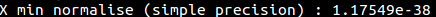
\includegraphics[scale=0.5]{XMinNormaliseSimple.png}
  							\caption{Valeur décimale affichée du $X_{min}$ normalisé simple}
					\end{figure}

			\subsection{$X_{min}$ normalisé en double précision}
				\subsubsection{Codage binaire}
					En codage $64$ bits, on a :
					\begin{figure}[!h]
						\centering
  							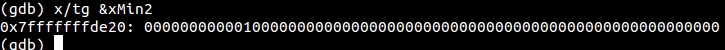
\includegraphics[scale=0.5]{BinaireXMinNormaliseDouble.png}
  							\caption{Codage binaire du $X_{min}$ normalisé en double précision}
					\end{figure}
	
					On en déduit donc que le nombre flottant, en double précision :
					\begin{itemize}
						\item est bien composé de $64$ bits;
						\item est positif (bit de signe à 0);
						\item est normalisé (l'exposant n'est pas codé par $00000000$);
						\item a un exposant dont le codage binaire est $00000000001$;
						\item a une mantisse dont le codage binaire est $00000000 00000000 0000000 0000000 00000000 00000000 0000$.
					\end{itemize}

				\subsubsection{Valeur exacte}
					On a, là aussi, clairement : 
					\begin{itemize}
						\item le bit de signe $s = 0$;
						\item la valeur de la mantisse qui vaut $m = 0$.
					\end{itemize}
					On a $(e)_{2} = (00000000001)_{2} = (e_{10}e_{9}…e_{0})_{2}$.\\
					On en déduit la valeur en base $10$, 
					\[\begin{aligned}
						e & = \sum_{i=0}^{10} e_{i}2^{i}\\
						  & = 2^{0}\\
						  & = 1
					\end{aligned}\]
					D'où $e-d = 1 - 1023 = -1022$.\\
					Finalement, la valeur $v$ du $X_{min}$ normalisé en double précision est :
					\[\begin{aligned}
						v & = (-1)^{0} \times 1.0 \times 2^{-1022}\\
						  & = 2^{-1022}
					\end{aligned}\]

				\subsubsection{Valeur décimale}
					On en déduit la valeur décimale suivante :
					\[\begin{aligned}
						v & = 2^{-1022}\\
						  & \approx 2.225 \times 10^{-308}
					\end{aligned}\]
					Ce qui confirme le résultat affiché à l'écran :
					\begin{figure}[!h]
						\centering
  							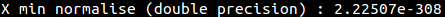
\includegraphics[scale=0.5]{XMinNormaliseDouble.png}
  							\caption{Valeur décimale affichée du $X_{min}$ normalisé double}
					\end{figure}
			    	
			\subsection{$X_{min}$ dénormalisé en simple précision}
				\subsubsection{Codage binaire}
					En codage $32$ bits, on a :
					\begin{figure}[!h]
						\centering
  							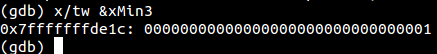
\includegraphics[scale=0.5]{BinaireXMinDenormaliseSimple.png}
  							\caption{Codage binaire du $X_{min}$ dénormalisé en simple précision}
					\end{figure}

					On en déduit donc que le nombre flottant, en simple précision :
					\begin{itemize}
						\item est bien composé de $32$ bits;
						\item est positif (bit de signe à 0);
						\item est bien normalisé (l'exposant est bien codé par $00000000$);
						\item a une mantisse dont le codage binaire est $00000000 00000000 000001$.
					\end{itemize}

				\subsubsection{Valeur exacte}
					On a maintenant : 
					\begin{itemize}
						\item le bit de signe $s = 0$;
						\item l'exposant qui ne vaut pas $-127$ comme on pourrait le penser mais bien $-126$ (cf introduction).
					\end{itemize}
					Trouvons la valeur de la mantisse en base $10$.
					On rajoute le bit implicite et alors on a $(m)_{2} = (0,00000000 00000000 000001)_{2}$, d'où :
					\[
						m = 2^{-23}
					\]
					Finalement, la valeur $v$ du $X_{min}$ dénormalisé en simple précision est :
					\[\begin{aligned}
						v & = (-1)^{0} \times 2^{-23} \times 2^{-126}\\
						  & = 2^{-149}
					\end{aligned}\]

				\subsubsection{Valeur décimale}
					On en déduit la valeur décimale suivante :
					\[\begin{aligned}
						v & = 2^{-149}\\
						  & \approx 1.401 \times 10^{-45}
					\end{aligned}\]
					Ce qui confirme le résultat affiché à l'écran :
					\begin{figure}[!h]
						\centering
  							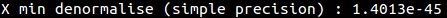
\includegraphics[scale=0.5]{XMinDenormaliseSimple.png}
  							\caption{Valeur décimale affichée du $X_{min}$ dénormalisé simple}
					\end{figure}

			\subsection{$X_{min}$ dénormalisé en double précision}
				\subsubsection{Codage binaire}
					En codage $64$ bits, on a :
					\begin{figure}[!h]
						\centering
  							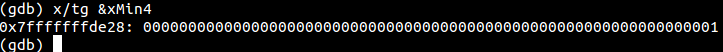
\includegraphics[scale=0.5]{BinaireXMinDenormaliseDouble.png}
  							\caption{Codage binaire du $X_{min}$ dénormalisé en double précision}
					\end{figure}

					On en déduit donc que le nombre flottant, en double précision :
					\begin{itemize}
						\item est bien composé de $64$ bits;
						\item est positif (bit de signe à 0);
						\item est bien dénormalisé (l'exposant est bien codé par $00000000$);
						\item a une mantisse dont le codage binaire est $00000000 00000000 0000000 0000000 00000000 00000000 0001$.
					\end{itemize}

				\subsubsection{Valeur exacte}
					On a maintenant : 
					\begin{itemize}
						\item le bit de signe $s = 0$;
						\item l'exposant qui ne vaut pas $-1023$ comme on pourrait le penser mais bien $-1022$ (cf introduction).
					\end{itemize}
					Trouvons la valeur de la mantisse en base $10$.
					On rajoute le bit implicite et alors on a $(m)_{2} = (0,00000000 00000000 0000000 0000000 00000000 00000000 0001)_{2}$, d'où :
					\[
						m = 2^{-52}
					\]
					Finalement, la valeur $v$ du $X_{min}$ dénormalisé en double précision est :
					\[\begin{aligned}
						v & = (-1)^{0} \times 2^{-52} \times 2^{-1022}\\
						  & = 2^{-1074}
					\end{aligned}\]

				\subsubsection{Valeur décimale}
					On en déduit la valeur décimale suivante :
					\[\begin{aligned}
						v & = 2^{-1074}\\
						  & \approx 4.940 \times 10^{-324}
					\end{aligned}\]
					Ce qui confirme le résultat affiché à l'écran :
					\begin{figure}[!h]
						\centering
  							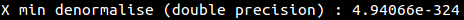
\includegraphics[scale=0.5]{XMinDenormaliseDouble.png}
  							\caption{Valeur décimale affichée du $X_{min}$ dénormalisé double}
					\end{figure}

		\section{$X_{max}$}
			$X_{max}$ est le plus grand nombre flottant que l'on peut coder sur machine.
			On développe un programme C pour pouvoir le calculer en normalisé et en dénormalisé :
			\lstinputlisting{"../Programmes/X max/src/xMax.c"}
			On va donc poser un break sur les lignes 61, 62, 63 et 64.

			Ce qui nous donne comme sortie à l'écran :
			\begin{figure}[!h]
				\centering
  					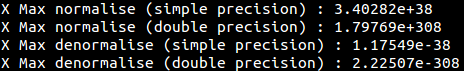
\includegraphics[scale=0.6]{XMax.png}
  					\caption{Résultat affiché par le programme}
			\end{figure}

			\subsection{$X_{max}$ normalisé en simple précision}
				\subsubsection{Codage binaire}
					En codage $32$ bits, on a :
					\begin{figure}[!h]
						\centering
  							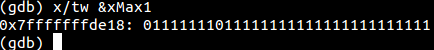
\includegraphics[scale=0.5]{BinaireXMaxNormaliseSimple.png}
  							\caption{Codage binaire du $X_{max}$ normalisé en simple précision}
					\end{figure}

					On en déduit donc que le nombre flottant, en simple précision :
					\begin{itemize}
						\item est bien composé de $32$ bits;
						\item est positif (bit de signe à 0);
						\item est bien dénormalisé (l'exposant n'est pas codé par $00000000$);
						\item a un exposant dont le codage binaire est $11111110$ (et non pas $11111111$, sinon ce serait infinity ou NaN);
						\item a une mantisse dont le codage binaire est $11111111 11111111 1111111$.
					\end{itemize}
					\newpage

				\subsubsection{Valeur exacte}
					On a : 
					\begin{itemize}
						\item le bit de signe $s = 0$;
					\end{itemize}
					Trouvons la valeur de l'exposant $e$.
					On a l'expression binaire de l'exposant $(e)_{2} = (11111110)_{2} = (e_{7}e_{6}…e_{0})_{2}$.\\
					On en déduit la valeur en base $10$, 
					\[\begin{aligned}
						e & = \sum_{i=0}^{7} e_{i}2^{i}\\
						  & = 2^{1} + 2^{2} + 2^{3}+ 2^{5}+ 2^{5}+ 2^{6} + 2^{7}\\
						  & = 2\times\frac{1 - 2^{7}}{1 - 2}\\
						  & = 254
					\end{aligned}\]
					D'où $e-d = 254 - 127 = 127$.\\
					Trouvons la valeur de la mantisse $m$.
					On a le codage binaire de la mantisse qui est : $(m)_{2} = (0,11111111 11111111 1111111)_{2} = (0,m_{1}m_{2}…m_{23})_{2}$.\\
					On en déduit la valeur en base $10$, 
					\[\begin{aligned}
						m & = \sum_{i=1}^{23} m_{i}2^{-i}\\
						  & = 2^{-23}\frac{1 - 2^{23}}{1 - 2}\\
						  & \approx 0.99999988079071044921875
					\end{aligned}\]
					D'où $1 + m = 1.99999988079071044921875$.\\
					Finalement, la valeur $v$ du $X_{max}$ normalisé en simple précision est :
					\[\begin{aligned}
						v & \approx (-1)^{0} \times 1.99999988079071044921875 \times 2^{127}\\
						  & = 1.99999988079071044921875 \times 2^{127}
					\end{aligned}\]

				\subsubsection{Valeur décimale}
					On en déduit la valeur décimale suivante :
					\[\begin{aligned}
						v & \approx 1.99999988079071044921875 \times 2^{127}\\
						  & \approx 3.40282346638528859811704183484516925440 \times 10^{38}
					\end{aligned}\]
					Ce qui confirme le résultat affiché à l'écran :
					\begin{figure}[!h]
						\centering
  							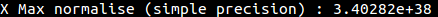
\includegraphics[scale=0.5]{XMaxNormaliseSimple.png}
  							\caption{Valeur décimale affichée du $X_{max}$ normalisé simple}
					\end{figure}
					\newpage

			\subsection{$X_{max}$ normalisé en double précision}
				\subsubsection{Codage binaire}
					En codage $64$ bits, on a :
					\begin{figure}[!h]
						\centering
  							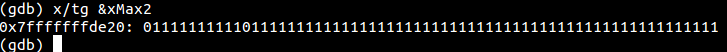
\includegraphics[scale=0.5]{BinaireXMaxNormaliseDouble.png}
  							\caption{Codage binaire du $X_{max}$ normalisé en double précision}
					\end{figure}
	
					On en déduit donc que le nombre flottant, en double précision :
					\begin{itemize}
						\item est bien composé de $64$ bits;
						\item est positif (bit de signe à 0);
						\item est bien normalisé (l'exposant n'est pas codé par $00000000$);
						\item a un exposant dont le codage binaire est $11111111110$;
						\item a une mantisse dont le codage binaire est $11111111 11111111 11111111 11111111 11111111 11111111 1111$.
					\end{itemize}

				\subsubsection{Valeur exacte}
					On a : 
					\begin{itemize}
						\item le bit de signe $s = 0$;
					\end{itemize}
					Trouvons la valeur de l'exposant $e$.
					On a l'expression binaire de l'exposant $(e)_{2} = (11111111110)_{2} = (e_{10}e_{9}…e_{0})_{2}$.\\
					On en déduit la valeur en base $10$, 
					\[\begin{aligned}
						e & = \sum_{i=0}^{10} e_{i}2^{i}\\
						  & = 2^{1} + 2^{2} + 2^{3}+ 2^{5}+ 2^{5}+ 2^{6} + 2^{7} + 2^{8} + 2^{9} + 2^{10}\\
						  & = 2\times\frac{1 - 2^{10}}{1 - 2}\\
						  & = 2046
					\end{aligned}\]
					D'où $e-d = 2046 - 1023 = 1023$.\\
					Trouvons la valeur de la mantisse $m$.
					On a le codage binaire de la mantisse qui est : $(m)_{2} = (0,11111111 11111111 11111111 11111111 11111111 11111111 1111)_{2} = (0,m_{1}m_{2}…m_{52})_{2}$.\\
					On en déduit la valeur en base $10$, 
					\[\begin{aligned}
						m & = \sum_{i=1}^{52} m_{i}2^{-i}\\
						  & = 2^{-52}\frac{1 - 2^{52}}{1 - 2}\\
						  & \approx 0.9999999999999997779553950749686919152736663818359375
					\end{aligned}\]
					D'où $1 + m \approx 1.9999999999999997779553950749686919152736663818359375$.\\
					Finalement, la valeur $v$ du $X_{max}$ normalisé en double précision est :
					\[\begin{aligned}
						v & \approx 1.9999999999999997779553950749686919152736663818359375 \times 2^{1023}\\
					\end{aligned}\]

				\subsubsection{Valeur décimale}
					On en déduit la valeur décimale suivante :
					\[\begin{aligned}
						v & \approx 1.9999999999999997779553950749686919152736663818359375 \times 2^{1023}\\
						  & \approx 1.797693134862315708145274237317043567980705675258449965 \times 10^{308}
					\end{aligned}\]
					Ce qui confirme le résultat affiché à l'écran :
					\begin{figure}[!h]
						\centering
  							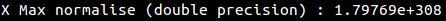
\includegraphics[scale=0.5]{XMaxNormaliseDouble.png}
  							\caption{Valeur décimale affichée du $X_{max}$ normalisé double}
					\end{figure}
			    	
			\subsection{$X_{max}$ dénormalisé en simple précision}
				\subsubsection{Codage binaire}
					En codage $32$ bits, on a :
					\begin{figure}[!h]
						\centering
  							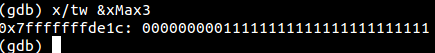
\includegraphics[scale=0.5]{BinaireXMaxDenormaliseSimple.png}
  							\caption{Codage binaire du $X_{max}$ dénormalisé en simple précision}
					\end{figure}

					On en déduit donc que le nombre flottant, en simple précision :
					\begin{itemize}
						\item est bien composé de $32$ bits;
						\item est positif (bit de signe à 0);
						\item est bien dénormalisé (l'exposant est bien codé par $00000000$);
						\item a une mantisse dont le codage binaire est $11111111 11111111 1111111$.
					\end{itemize}

				\subsubsection{Valeur exacte}
					On a maintenant : 
					\begin{itemize}
						\item le bit de signe $s = 0$;
						\item l'exposant qui ne vaut pas $-127$ comme on pourrait le penser mais bien $-126$ (cf introduction).
					\end{itemize}
					Trouvons la valeur de la mantisse en base $10$.
					On rajoute le bit implicite et alors on a $(m)_{2} = (0,11111111 11111111 1111111)_{2} = (0,m_{1}m_{2}…m_{23})_{2}$, d'où :
					\[\begin{aligned}
						m & = \sum_{i=1}^{23} m_{i}2^{-i}\\
						  & = 2^{-23}\frac{1 - 2^{23}}{1 - 2}\\
						  & \approx 0.99999988079071044921875
					\end{aligned}\]
					Finalement, la valeur $v$ du $X_{max}$ dénormalisé en simple précision est :
					\[\begin{aligned}
						v & \approx 0.99999988079071044921875 \times 2^{-126}
					\end{aligned}\]

				\subsubsection{Valeur décimale}
					On en déduit la valeur décimale suivante :
					\[\begin{aligned}
						v & \approx 0.99999988079071044921875 \times 2^{-126}\\
						  & \approx 1.17549421069244107548702944 \times 10^{-38}
					\end{aligned}\]
					Ce qui confirme le résultat affiché à l'écran :
					\begin{figure}[!h]
						\centering
  							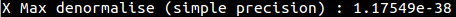
\includegraphics[scale=0.5]{XMaxDenormaliseSimple.png}
  							\caption{Valeur décimale affichée du $X_{max}$ dénormalisé simple}
					\end{figure}

			\subsection{$X_{max}$ dénormalisé en double précision}
				\subsubsection{Codage binaire}
					En codage $32$ bits, on a :
					\begin{figure}[!h]
						\centering
  							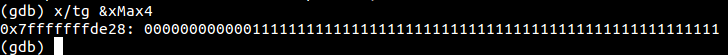
\includegraphics[scale=0.5]{BinaireXMaxDenormaliseDouble.png}
  							\caption{Codage binaire du $X_{max}$ dénormalisé en double précision}
					\end{figure}

					On en déduit donc que le nombre flottant, en double précision :
					\begin{itemize}
						\item est bien composé de $32$ bits;
						\item est positif (bit de signe à 0);
						\item est bien dénormalisé (l'exposant est bien codé par $00000000000$);
						\item a une mantisse dont le codage binaire est $11111111 11111111 11111111 11111111 11111111 11111111 1111$.
					\end{itemize}

				\subsubsection{Valeur exacte}
					On a maintenant : 
					\begin{itemize}
						\item le bit de signe $s = 0$;
						\item l'exposant qui ne vaut pas $-1023$ comme on pourrait le penser mais bien $-1022$ (cf introduction).
					\end{itemize}
					Trouvons la valeur de la mantisse en base $10$.
					On rajoute le bit implicite et alors on a $(m)_{2} = (0,11111111 11111111 11111111 11111111 11111111 11111111 1111)_{2} = (0,m_{1}m_{2}…m_{52})_{2}$, d'où :
					\[\begin{aligned}
						m & = \sum_{i=1}^{52} m_{i}2^{-i}\\
						  & = 2^{-52}\frac{1 - 2^{52}}{1 - 2}\\
						  & \approx 0.9999999999999997779553950749686919152736663818359375
					\end{aligned}\]
					Finalement, la valeur $v$ du $X_{max}$ dénormalisé en double précision est :
					\[\begin{aligned}
						v & \approx 0.9999999999999997779553950749686919152736663818359375 \times 2^{-1022}
					\end{aligned}\]

				\subsubsection{Valeur décimale}
					On en déduit la valeur décimale suivante :
					\[\begin{aligned}
						v & \approx 0.9999999999999997779553950749686919152736663818359375 \times 2^{-1022}\\
						  & \approx 2.225074 \times 10^{-308}
					\end{aligned}\]
					Ce qui confirme le résultat affiché à l'écran :
					\begin{figure}[!h]
						\centering
  							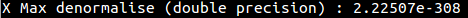
\includegraphics[scale=0.5]{XMaxDenormaliseDouble.png}
  							\caption{Valeur décimale affichée du $X_{max}$ dénormalisé double}
					\end{figure}

		\section{Le zéro et l'unité}
			On s'intéresse ici à des nombres très important car ils sont constamment utilisés en calcul scientifique.
			Il s'agit bien des éléments neutres des lois de compositions du corps des réels : $0$ pour l'addition et $1$ pour la multiplication.
			On développe un programme C pour pouvoir les afficher :
			\lstinputlisting{"../Programmes/0 et 1/src/zeroEtUn.c"}
			On va donc poser un break sur les lignes 9, 10, 11 et 12.

			Ce qui nous donne comme sortie à l'écran :
			\begin{figure}[!h]
				\centering
  					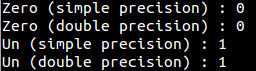
\includegraphics[scale=0.6]{ZeroEtUn.png}
  					\caption{Résultat affiché par le programme}
			\end{figure}
			\newpage

			\subsection{Le zéro machine en simple précision}
				\subsubsection{Codage binaire}
					En codage $32$ bits, on a :
					\begin{figure}[!h]
						\centering
  							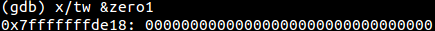
\includegraphics[scale=0.5]{BinaireZeroMachineSimple.png}
  							\caption{Codage binaire du zéro machine en simple précision}
					\end{figure}

					On en déduit donc que le nombre flottant, en simple précision :
					\begin{itemize}
						\item est bien composé de $32$ bits;
						\item est positif (bit de signe à 0), mais il existe une autre valeur du zéro qui est négative (bit de signe à 1) qui est traitée par la machine comme étant la même valeur;
						\item est dénormalisé (l'exposant est codé par $00000000$);
						\item a une mantisse dont le codage binaire est $00000000 00000000 0000000$.
					\end{itemize}

				\subsubsection{Valeur exacte}
					On a maintenant : 
					\begin{itemize}
						\item le bit de signe $s = 0$ ou $s = 1$ (peu importe);
						\item l'exposant qui vaut $-126$ car le nombre est dénormalisé;
						\item la mantisse qui vaut $0$.
					\end{itemize}
					Finalement, la valeur $v$ du zéro machine en simple précision est :
					\[\begin{aligned}
						v & = \pm 0.0 \times 2^{-126}\\
					\end{aligned}\]

				\subsubsection{Valeur décimale}
					On en déduit la valeur décimale suivante :
					\[\begin{aligned}
						v & = \pm 0.0 \times 2^{-126}\\
						  & = 0
					\end{aligned}\]
					Clairement confirmée par notre programme :
					\begin{figure}[!h]
						\centering
  							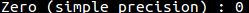
\includegraphics[scale=0.5]{ZeroMachineSimple.png}
  							\caption{Valeur décimale affichée du zéro machine en simple précision}
					\end{figure}

			\subsection{Le zéro machine en double précision}
				\subsubsection{Codage binaire}
					En codage $64$ bits, on a :
					\begin{figure}[!h]
						\centering
  							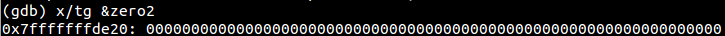
\includegraphics[scale=0.5]{BinaireZeroMachineDouble.png}
  							\caption{Codage binaire du zéro machine en double précision}
					\end{figure}

					On en déduit donc que le nombre flottant, en simple précision :
					\begin{itemize}
						\item est bien composé de $64$ bits;
						\item est positif (bit de signe à 0), mais il existe une autre valeur du zéro qui est négative (bit de signe à 1) qui est traitée par la machine comme étant la même valeur;
						\item est dénormalisé (l'exposant est codé par $00000000000$);
						\item a une mantisse dont le codage binaire est $00000000 00000000 00000000 00000000 00000000 00000000 00000$.
					\end{itemize}

				\subsubsection{Valeur exacte}
					On a maintenant : 
					\begin{itemize}
						\item le bit de signe $s = 0$ ou $s = 1$ (peu importe);
						\item l'exposant qui vaut $-1022$ car le nombre est dénormalisé;
						\item la mantisse qui vaut $0$.
					\end{itemize}
					Finalement, la valeur $v$ du zéro machine en simple précision est :
					\[\begin{aligned}
						v & = \pm 0.0 \times 2^{-1022}\\
					\end{aligned}\]

				\subsubsection{Valeur décimale}
					On en déduit la valeur décimale suivante :
					\[\begin{aligned}
						v & = \pm 0.0 \times 2^{-1022}\\
						  & = 0
					\end{aligned}\]
					Clairement confirmée par notre programme :
					\begin{figure}[!h]
						\centering
  							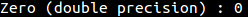
\includegraphics[scale=0.5]{ZeroMachineDouble.png}
  							\caption{Valeur décimale affichée du zéro machine en double précision}
					\end{figure}
			    	
			\subsection{L'unité machine en simple précision}
				\subsubsection{Codage binaire}
					En codage $32$ bits, on a :
					\begin{figure}[!h]
						\centering
  							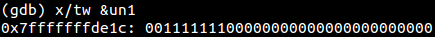
\includegraphics[scale=0.5]{BinaireUnMachineSimple.png}
  							\caption{Codage binaire de l'unité machine en simple précision}
					\end{figure}

					On en déduit donc que le nombre flottant, en simple précision :
					\begin{itemize}
						\item est bien composé de $32$ bits;
						\item est bien positif (bit de signe à 0);
						\item est normalisé;
						\item a un exposant dont le codage binaire est $01111111$;
						\item a une mantisse dont le codage binaire est $00000000 00000000 0000000$.
					\end{itemize}

				\subsubsection{Valeur exacte}
					On a maintenant : 
					\begin{itemize}
						\item le bit de signe qui est $s = 0$;
						\item la mantisse qui vaut $0$, donc $1+m = 1$.
					\end{itemize}
					La valeur de l'exposant est l'expression décimale du nombre binaire $(e)_{2} = (01111111)_{2} = (e_{7}e_{6}…e_{0})_{2}$ :
					\[\begin{aligned}
						e & = \sum_{i=0}^{7} e_{i}2^{i}\\
						  & = \frac{1 - 2^{7}}{1 - 2}\\
						  & = 127
					\end{aligned}\]
					D'où $e - d = 127 - 127 = 0$.
					Finalement, la valeur $v$ de l'unité machine en simple précision est :
					\[\begin{aligned}
						v & = 1 \times 2^{0}\\
					\end{aligned}\]

				\subsubsection{Valeur décimale}
					On en déduit la valeur décimale suivante :
					\[\begin{aligned}
						v & = 1 \times 2^{0}\\
						  & = 1
					\end{aligned}\]
					Clairement confirmée par notre programme :
					\begin{figure}[!h]
						\centering
  							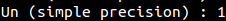
\includegraphics[scale=0.5]{UnMachineSimple.png}
  							\caption{Valeur décimale affichée de l'unité machine en simple précision}
					\end{figure}

			\subsection{L'unité machine en double précision}
				\subsubsection{Codage binaire}
					En codage $64$ bits, on a :
					\begin{figure}[!h]
						\centering
  							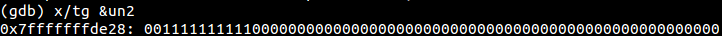
\includegraphics[scale=0.5]{BinaireUnMachineDouble.png}
  							\caption{Codage binaire de l'unité machine en double précision}
					\end{figure}

					On en déduit donc que le nombre flottant, en double précision :
					\begin{itemize}
						\item est bien composé de $64$ bits;
						\item est bien positif (bit de signe à 0);
						\item est normalisé;
						\item a un exposant dont le codage binaire est $01111111111$;
						\item a une mantisse dont le codage binaire est $00000000 00000000 00000000 00000000 00000000 00000000 00000$.
					\end{itemize}

				\subsubsection{Valeur exacte}
					On a maintenant : 
					\begin{itemize}
						\item le bit de signe qui est $s = 0$;
						\item la mantisse qui vaut $0$, donc $1+m = 1$.
					\end{itemize}
					La valeur de l'exposant est l'expression décimale du nombre binaire $(e)_{2} = (01111111111)_{2} = (e_{10}e_{9}…e_{0})_{2}$ :
					\[\begin{aligned}
						e & = \sum_{i=0}^{10} e_{i}2^{i}\\
						  & = \frac{1 - 2^{10}}{1 - 2}\\
						  & = 1023
					\end{aligned}\]
					D'où $e - d = 1023 - 1023 = 0$.
					Finalement, la valeur $v$ de l'unité machine en double précision est :
					\[\begin{aligned}
						v & = 1 \times 2^{0}\\
					\end{aligned}\]

				\subsubsection{Valeur décimale}
					On en déduit la valeur décimale suivante :
					\[\begin{aligned}
						v & = 1 \times 2^{0}\\
						  & = 1
					\end{aligned}\]
					Clairement confirmée par notre programme :
					\begin{figure}[!h]
						\centering
  							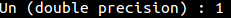
\includegraphics[scale=0.5]{UnMachineDouble.png}
  							\caption{Valeur décimale affichée de l'unité machine en double précision}
					\end{figure}

	\chapter{Le nombre flottant $0.1$}
		Dans cette partie, on étudie le flottant $0.1$ et nous allons voir que certaines constantes sont inexactes…
		On développe un programme C pour pouvoir l'afficher :
		\lstinputlisting{"../Programmes/0.1/src/zeroUn.c"}
		On va donc poser un break sur les lignes 7 et 8.

		Ce qui nous donne comme sortie à l'écran :
		\begin{figure}[!h]
			\centering
  				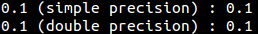
\includegraphics[scale=0.6]{ZeroUn.png}
  				\caption{Résultat affiché par le programme}
		\end{figure}

		\section{Le $0.1$ machine en simple précision}
			\subsection{Codage binaire}
				En codage $32$ bits, on a :
				\begin{figure}[!h]
					\centering
  						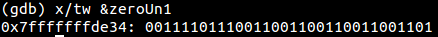
\includegraphics[scale=0.5]{BinaireZeroUnSimple.png}
  						\caption{Codage binaire du $0.1$ machine en simple précision}
				\end{figure}

				On en déduit donc que le nombre flottant, en simple précision :
				\begin{itemize}
					\item est bien composé de $32$ bits;
					\item est bien positif (bit de signe à 0);
					\item est normalisé (l'exposant n'est pas codé par $00000000$);
					\item a un exposant dont le codage binaire est $01111011$.
					\item a une mantisse dont le codage binaire est $10011001 10011001 1001101$.
				\end{itemize}

			\subsection{Valeur exacte}
				On a maintenant : 
				\begin{itemize}
					\item le bit de signe $s = 0$;
				\end{itemize}
				La valeur de l'exposant est l'expression décimale du nombre binaire $(e)_{2} = (01111011)_{2} = (e_{7}e_{6}…e_{0})_{2}$ :
				\[\begin{aligned}
					e & = \sum_{i=0}^{7} e_{i}2^{i}\\
				 	  & = 2^{0} + 2^{1} + 2^{3} + 2^{4} + 2^{5} + 2^{6}\\
				 	  & = 123
				\end{aligned}\]
				D'où $e - d = 123 - 127 = -4$
				La valeur de la mantisse est l'expression décimale du nombre binaire $(m)_{2} = (0, 10011001 10011001 1001101)_{2} = (0,m_{1}m_{2}…m_{23})_{2}$ :
				\[\begin{aligned}
					m & = \sum_{i=1}^{23} m_{i}2^{-i}\\
					  & = 2^{-1} + 2^{-4} + 2^{-5} + 2^{-8} + 2^{-9} + 2^{-12} + 2^{-13} + 2^{-16} + 2^{-17} + 2^{-20} + 2^{-21} + 2^{-23}\\
					  & \approx 0.60000002384
				\end{aligned}\]
				D'où $1 + m \approx 1.60000002384$.
				Finalement, la valeur $v$ du $0.1$ machine en simple précision est :
				\[\begin{aligned}
					v & \approx 1.60000002384 \times 2^{-4}\\
				\end{aligned}\]

			\subsection{Valeur décimale}
				On en déduit la valeur décimale suivante :
				\[\begin{aligned}
					v & \approx 1.60000002384 \times 2^{-4}\\
					  & \approx 0.10000000149
				\end{aligned}\]
				Ce qui n'est, ni la valeur exacte recherchée, ni la valeur affichée par notre programme :
				\begin{figure}[!h]
					\centering
  						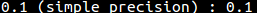
\includegraphics[scale=0.5]{ZeroUnSimple.png}
  						\caption{Valeur décimale affichée du $0.1$ machine en simple précision}
				\end{figure}

				En fait, une approximation de $0.1$ a été faite par la machine car l'expression de la mantisse en notation binaire scientifique est infinie : elle suit un schéma régulier qui se répète indéfiniment.
				Pour avoir une valeur exacte en binaire, il nous faudrait une quantité infinie de bits sur la mantisse pour pouvoir le stocker sans l'approximer $(m)_{2} = (0,1001 \ 1001 \ 1001…)_{2} = 0.6$.
				En effet, $1.6 \times 2^{-4} = 0.1$.
				La machine affiche bien $0.1$ car elle fait elle-même l'approximation à l'affichage que $0.10000000149 \approx 0.1$, mais si on lui demande d'afficher la variable avec $50$ décimales (avec \%.50f dans le printf), on a bien :
				\begin{figure}[!h]
					\centering
  						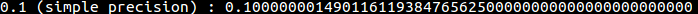
\includegraphics[scale=0.5]{ZeroUnSimple50Decimales.png}
  						\caption{Affichage de 50 décimales du $0.1$ machine en simple précision}
				\end{figure}
				\newpage

		\section{Le $0.1$ machine en double précision}
			\subsection{Codage binaire}
				En codage $64$ bits, on a :
				\begin{figure}[!h]
					\centering
  						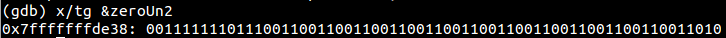
\includegraphics[scale=0.5]{BinaireZeroUnDouble.png}
  						\caption{Codage binaire du $0.1$ machine en double précision}
				\end{figure}

				On en déduit donc que le nombre flottant, en double précision :
				\begin{itemize}
					\item est bien composé de $64$ bits;
					\item est bien positif (bit de signe à 0);
					\item est normalisé (l'exposant n'est pas codé par $00000000$);
					\item a un exposant dont le codage binaire est $01111111011$.
					\item a une mantisse dont le codage binaire est $10011001 10011001 10011001 10011001 10011001 10011001 1010$.
				\end{itemize}

			\subsection{Valeur exacte}
				On a maintenant : 
				\begin{itemize}
					\item le bit de signe $s = 0$;
				\end{itemize}
				La valeur de l'exposant est l'expression décimale du nombre binaire $(e)_{2} = (01111111011)_{2} = (e_{10}e_{9}…e_{0})_{2}$ :
				\[\begin{aligned}
					e & = \sum_{i=0}^{10} e_{i}2^{i}\\
					  & = 2^{0} + 2^{1} + 2^{3} + 2^{4} + 2^{5} + 2^{6} + 2^{7} + 2^{8} + 2^{9}\\
					  & = 1019
				\end{aligned}\]
				D'où $e - d = 1019 - 1023 = -4$
				La valeur de la mantisse est l'expression décimale du nombre binaire $(m)_{2} = (0, 10011001 10011001 10011001 10011001 10011001 10011001 1010)_{2} = (0,m_{1}m_{2}…m_{52})_{2}$ :
				\[\begin{aligned}
					m & = \sum_{i=1}^{52} m_{i}2^{-i}\\
					  & = 2^{-1} + 2^{-4} + 2^{-5} + 2^{-8} + … + 2^{-45} + 2^{-48} + 2^{-49} + 2^{-51}\\
					  & \approx 0.600000000000000088817841970012523233890533447265625
				\end{aligned}\]
				D'où $1 + m \approx 1.6$.
				Finalement, la valeur $v$ du $0.1$ machine en double précision est :
				\[\begin{aligned}
					v & \approx 1.600000000000000088817841970012523233890533447265625\times 2^{-4}\\
				\end{aligned}\]
				\newpage

			\subsection{Valeur décimale}
				On en déduit la valeur décimale suivante :
				\[\begin{aligned}
					v & \approx 1.600000000000000088817841970012523233890533447265625 \times 2^{-4}\\
					  & \approx 0.1000000000000000055511151231257827021181583404541015625
				\end{aligned}\]
				On a bien la même approximation à l'affichage (à cause du \%g dans le printf) qui est réalisée :
				\begin{figure}[!h]
					\centering
  						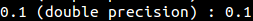
\includegraphics[scale=0.5]{ZeroUnDouble.png}
  						\caption{Valeur décimale affichée du $0.1$ machine en double précision}
				\end{figure}

				L'approximation est bien plus précise ici, si l'on affiche la variable avec $50$ décimales (avec \%.50f dans le printf), on a bien :
				\begin{figure}[!h]
					\centering
  						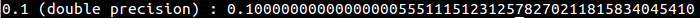
\includegraphics[scale=0.5]{ZeroUnDouble50Decimales.png}
  						\caption{Affichage de 50 décimales du $0.1$ machine en double précision}
				\end{figure}


	\chapter{Étude d'une somme de termes inférieurs à l'$\epsilon_{machine}$}
		Dans cette partie, on se propose d'étudier une somme de termes inférieurs à l'epsilon machine.
		On se donne un nombre flottant $Y \in ]0;\epsilon_{machine}[$ et on va s'intéresser à $Z = \sum_{i = 1}^{n} Y$ pour certaines valeurs de $n \in \mathbb{N}^{*}$.
		On prend $Y = 2^{-55} \approx 2.7755576 \times10^{-17}$ car ce nombre est inférieur à l'epsilon machine strictement en simple et double précision et il est supérieur au zéro machine et normalisé en simple et double précision.
		On développe un programme C pour pouvoir calculer cette somme :
		\lstinputlisting{"../Programmes/Somme epsilon/src/somme.c"}
		On va donc poser un break sur les lignes 40 à 47.

		Ce qui nous donne comme sortie à l'écran :
		\begin{figure}[!h]
			\centering
  				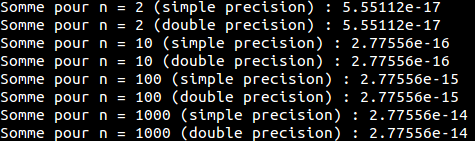
\includegraphics[scale=0.6]{Somme.png}
  				\caption{Résultat affiché par le programme}
		\end{figure}

		\section{Pour une somme de 2 termes}
			\subsection{Codage binaire}
				Pour ce qui est du codage binaire, on a en simple et double précision :
				\begin{figure}[!h]
					\centering
  						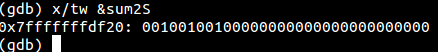
\includegraphics[scale=0.5]{BinaireSomme2Simple.png}
  						\caption{Somme de 2 termes en simple précision}
				\end{figure}
				\begin{figure}[!h]
					\centering
  						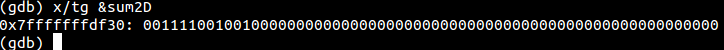
\includegraphics[scale=0.5]{BinaireSomme2Double.png}
  						\caption{Somme de 2 termes en double précision}
				\end{figure}

				Clairement, les nombres sont normalisés.

			\subsection{Valeur exacte}
				On devrait avoir :
				\[
					2\times2^{-55} = 2^{-54} 
				\]
				Pour les deux précisions, on remarque que le bit de signe est $0$ ($s = 0$), et que $m = 0$ (tout les bits de la mantisse sont à zéros).
				On a pour l'exposant en simple précision $(e)_{2} = (01001001)_{2}$.
				D'où :
				\[\begin{aligned}
					e & = 1 + 8 + 64
					  & = 73
				\end{aligned}\]
				Ainsi $e - d = 73 - 127 = -54$.
				Finalement on a bien en simple précision
				\[
					\sum_{i=1}^{2} Y = 1.0\times2^{-54} = 2^{-54}
				\]
				De même, en double précision, $(e)_{2} = (01111001001)_{2}$.
				D'où :
				\[\begin{aligned}
					e & = 1 + 8 + 64 + 128 + 256 + 512
					  & = 969
				\end{aligned}\]
				Ce qui implique que $e - d = 969 - 1023 = -54$.
				On a donc aussi en double précision :
				\[
					\sum_{i=1}^{2} Y = 1.0\times2^{-54} = 2^{-54}
				\]

			\subsection{Valeur décimale}
				On a en simple et double précision :
				\[\begin{aligned}
					\sum_{i=1}^{2} Y & = 2^{-54}\\
									 & \approx 5.5511151\times10^{-17}
				\end{aligned}\]
				Ce qui est confirmé à l'affichage :
				\begin{figure}[!h]
					\centering
  						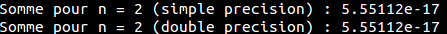
\includegraphics[scale=0.5]{Somme2.png}
  						\caption{Somme de 2 termes affichée en simple et double précision}
				\end{figure}

		\section{Pour une somme de 10 termes}
			\subsection{Codage binaire}
				Pour ce qui est du codage binaire, on a en simple et double précision :
				\begin{figure}[!h]
					\centering
  						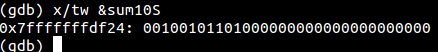
\includegraphics[scale=0.5]{BinaireSomme10Simple.png}
  						\caption{Somme de 10 termes en simple précision}
				\end{figure}
				\begin{figure}[!h]
					\centering
  						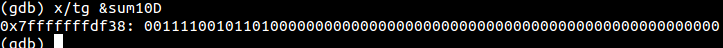
\includegraphics[scale=0.5]{BinaireSomme10Double.png}
  						\caption{Somme de 10 termes en double précision}
				\end{figure}

				Clairement, les nombres sont normalisés.

			\subsection{Valeur exacte}
				On devrait avoir :
				\[
					10\times2^{-55} = 5\times2^{-54} = 2.5\times2^{-53} = 1.25\times2^{-52} 
				\]
				Pour les deux précisions, on remarque que le bit de signe est $0$ ($s = 0$).
				On a pour l'exposant en simple précision $(e)_{2} = (01001011)_{2}$.
				D'où :
				\[\begin{aligned}
					e & = 1 + 2 + 8 + 64
					  & = 75
				\end{aligned}\]
				Ainsi $e - d = 75 - 127 = -52$.
				Et, $(m)_{2} = (0,0100000…)_{2}$
				D'où :
				\[\begin{aligned}
					m & = 2^{-2}
					  & = 0.25
				\end{aligned}\]
				Finalement on a bien en simple précision
				\[
					\sum_{i=1}^{10} Y = 1.25\times2^{-52}
				\]
				De même, en double précision, $(e)_{2} = (01111001011)_{2}$
				D'où :
				\[\begin{aligned}
					e & = 1 + 2 + 8 + 64 + 128 + 256 + 512
					  & = 971
				\end{aligned}\]
				Ce qui implique que $e - d = 971 - 1023 = -52$.
				Et, $(m)_{2} = (0,0100000…)_{2}$
				D'où :
				\[\begin{aligned}
					m & = 2^{-2}
					  & = 0.25
				\end{aligned}\]
				On a donc aussi en double précision :
				\[
					\sum_{i=1}^{10} Y = 1.25\times2^{-52}
				\]

			\subsection{Valeur décimale}
				On a en simple et double précision :
				\[\begin{aligned}
					\sum_{i=1}^{10} Y & = 1.25\times2^{-52}\\
									 & \approx 2.7755576\times10^{-16}
				\end{aligned}\]
				Ce qui est confirmé à l'affichage :
				\begin{figure}[!h]
					\centering
  						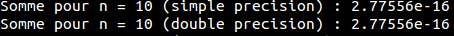
\includegraphics[scale=0.5]{Somme10.png}
  						\caption{Somme de 10 termes affichée en simple et double précision}
				\end{figure}
				\newpage

		\section{Pour une somme de 100 termes}
			\subsection{Codage binaire}
				Pour ce qui est du codage binaire, on a en simple et double précision :
				\begin{figure}[!h]
					\centering
  						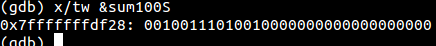
\includegraphics[scale=0.5]{BinaireSomme100Simple.png}
  						\caption{Somme de 100 termes en simple précision}
				\end{figure}
				\begin{figure}[!h]
					\centering
  						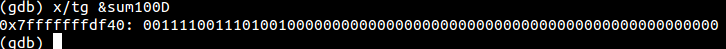
\includegraphics[scale=0.5]{BinaireSomme100Double.png}
  						\caption{Somme de 100 termes en double précision}
				\end{figure}

				Clairement, les nombres sont normalisés.

			\subsection{Valeur exacte}
				On devrait avoir :
				\[
					100\times2^{-55} = 10\times1.25\times2^{-52} = (1.25)^2\times2^{-49} = 1.5625\times2^{-49}
				\]
				Pour les deux précisions, on remarque que le bit de signe est $0$ ($s = 0$).
				On a pour l'exposant en simple précision $(e)_{2} = (01001110)_{2}$.
				D'où :
				\[\begin{aligned}
					e & = 2 + 4 + 8 + 64
					  & = 78
				\end{aligned}\]
				Ainsi $e - d = 78 - 127 = -49$.
				Et, $(m)_{2} = (0,100100000…)_{2}$
				D'où :
				\[\begin{aligned}
					m & = 2^{-1} + 2^{-4} 
					  & = 0.5 + 0.0625
					  & = 0,5625
				\end{aligned}\]
				Finalement on a bien en simple précision
				\[
					\sum_{i=1}^{100} Y = 1.5625\times2^{-49}
				\]
				De même, en double précision, $(e)_{2} = (01111001110)_{2}$
				D'où :
				\[\begin{aligned}
					e & = 2 + 4 + 8 + 64 + 128 + 256 + 512
					  & = 974
				\end{aligned}\]
				Ce qui implique que $e - d = 974 - 1023 = -49$.
				Et, $(m)_{2} = (0,1001000…)_{2}$
				D'où :
				\[\begin{aligned}
					m & = 0.5 + 0.0625
					  & = 0,5625
				\end{aligned}\]
				On a donc aussi en double précision :
				\[
					\sum_{i=1}^{100} Y = 1.5625\times2^{-49}
				\]

			\subsection{Valeur décimale}
				On a en simple et double précision :
				\[\begin{aligned}
				  \sum_{i=1}^{100} Y & = 1.5625\times2^{-49}\\
									 & \approx 2.77555756156\times10^{-15}
				\end{aligned}\]
				Ce qui est confirmé à l'affichage :
				\begin{figure}[!h]
					\centering
  						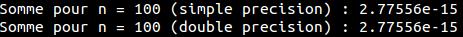
\includegraphics[scale=0.5]{Somme100.png}
  						\caption{Somme de 100 termes affichée en simple et double précision}
				\end{figure}

		\section{Pour une somme de 1000 termes}
			\subsection{Codage binaire}
				Pour ce qui est du codage binaire, on a en simple et double précision :
				\begin{figure}[!h]
					\centering
  						\includegraphics[scale=0.5]{BinaireSomme1000Simple.png}
  						\caption{Somme de 1000 termes en simple précision}
				\end{figure}
				\begin{figure}[!h]
					\centering
  						\includegraphics[scale=0.5]{BinaireSomme1000Double.png}
  						\caption{Somme de 1000 termes en double précision}
				\end{figure}

				Clairement, les nombres sont normalisés.

			\subsection{Valeur exacte}
				On devrait avoir :
				\[
					1000\times2^{-55} = 10\times1.5625\times2^{-49} = 1.25\times1.5625\times2^{-46} = 1.953125\times2^{-46}
				\]
				Pour les deux précisions, on remarque que le bit de signe est $0$ ($s = 0$).
				On a pour l'exposant en simple précision $(e)_{2} = (01010001)_{2}$.
				D'où :
				\[\begin{aligned}
					e & = 1 + 16 + 64
					  & = 81
				\end{aligned}\]
				Ainsi $e - d = 81 - 127 = -46$.
				Et, $(m)_{2} = (0,11110100…)_{2}$
				D'où :
				\[\begin{aligned}
					m & = 2^{-1} + 2^{-2} + 2^{-3} + 2^{-4} + 2^{-6}
					  & = 0.953125
				\end{aligned}\]
				Finalement on a bien en simple précision
				\[
					\sum_{i=1}^{1000} Y = 1.953125\times2^{-46}
				\]
				De même, en double précision, $(e)_{2} = (01111010001)_{2}$
				D'où :
				\[\begin{aligned}
					e & = 1 + 16 + 64 + 128 + 256 + 512
					  & = 977
				\end{aligned}\]
				Ce qui implique que $e - d = 977 - 1023 = -46$.
				Et, $(m)_{2} = (0,11110100…)_{2}$
				D'où :
				\[\begin{aligned}
					m & = 0.953125
				\end{aligned}\]
				On a donc aussi en double précision :
				\[
					\sum_{i=1}^{1000} Y = 1.953125\times2^{-46}
				\]

			\subsection{Valeur décimale}
				On a en simple et double précision :
				\[\begin{aligned}
				  \sum_{i=1}^{1000} Y & = 1.953125\times2^{-46}\\
									  & \approx 2.77555756156\times10^{-14}
				\end{aligned}\]
				Ce qui est confirmé à l'affichage :
				\begin{figure}[!h]
					\centering
  						\includegraphics[scale=0.5]{Somme1000.png}
  						\caption{Somme de 1000 termes affichée en simple et double précision}
				\end{figure}

		\section{Remarque : pour $n$ assez grand}
			Pour un $n$ assez grand (de l'ordre de la centaine de milliers de milliards de milliards), on aurait eu une somme qui atteint $1$.
			Et alors, on pourrait penser que $Z$ se stabilise à 1 par définition du $\epsilon_{machine}$.
			En effet, si l'on choisit plutot $Y = 2^{-24}$ et que l'on effectue $10^8$ fois la somme :
			\lstinputlisting{"../Programmes/Somme epsilon 1/src/somme.c"}

			On a comme sortie à l'écran :
			\begin{figure}[!h]
				\centering
  					\includegraphics[scale=0.4]{Somme1.png}
  					\caption{Résultat affiché par le programme}
			\end{figure}

			Et comme $Y$ est strictement inférieur au $\epsilon_{machine}$ simple, il est normal de trouver $1$ exactement pour la somme en simple précision et quelque chose de strictement plus grand que $1$ pour la somme en double.
			En effet, en double précision on a bien :
			\[
				10^{8}\times2^{-24} = (1.25)^{8}\times2^{0} \approx 5.96046447754
			\]
			D'où les codes binaires (on reconnait bien l'unité machine et on peut vérifier le résultat en double par un calcul similaire aux précédents) :
			\begin{figure}[!h]
				\centering
  					\includegraphics[scale=0.6]{BinaireSomme1.png}
  					\caption{Codes binaires des deux variables précédentes}
			\end{figure}

			Au vu de ces résultats, il nous semble logique de penser que la prochaine partie nous donnera comme résultat $1$ pour toute valeurs de $n$.


	\chapter{Ajout de l'unité à une somme de termes inférieurs à l'$\epsilon_{machine}$}
		On s'intéresse maintenant au résultat de l'ajout de 1 à la somme précédente.
		On va donc regarder la valeur de $1 + Z$.
		On produit un programme C pour pouvoir calculer cette somme :
		\lstinputlisting{"../Programmes/1 plus somme epsilon/src/somme.c"}
		On va donc poser un break sur les lignes 40 à 47.

		Ce qui nous donne comme sortie à l'écran :
		\begin{figure}[!h]
			\centering
  				\includegraphics[scale=0.4]{1PlusSomme.png}
  				\caption{Résultat affiché par le programme}
		\end{figure}

		Hérésie !
		Par définition de l'epsilon machine on devrait avoir $(…(((1 + y) + y) + y) + y …) = 1$.
		Or, on remarque que les valeurs de $Z$ pour lesquelles la somme dépasse l'epsilon machine en double précision nous donne $1 + Z > 1$.
		En fait, cela nous montre la non-associativité de l'additivité machine, car sinon on aurait $(…(((1 + y) + y) + y) + y …) = 1 + Z = 1$ peu importe si la valeur de $Z$ dépasse l'epsilon machine !

		\section{Pour une somme de 2 termes}
			Le code binaire confirme que le résultat trouvé pour les deux sommes (en simple et double précision) est le $1$ machine.
			\begin{figure}[!h]
				\centering
  					\includegraphics[scale=0.5]{Binaire1PlusSomme2Simple.png}
  					\caption{$1 + Z$ pour $n = 2$ en simple précision}
			\end{figure}
			\begin{figure}[!h]
				\centering
  					\includegraphics[scale=0.5]{Binaire1PlusSomme2Double.png}
  					\caption{$1 + Z$ pour $n = 2$ en double précision}
			\end{figure}

		\section{Pour les autres sommes}
			Clairement, on retrouve l'unité machine en simple précision, on s'intéressera donc à la double précision.
			\begin{figure}[!h]
				\centering
  					\includegraphics[scale=0.5]{Binaire1PlusSomme10Double.png}
  					\caption{$1 + Z$ pour $n = 10$ en double précision}
			\end{figure}
			\begin{figure}[!h]
				\centering
  					\includegraphics[scale=0.5]{Binaire1PlusSomme100Double.png}
  					\caption{$1 + Z$ pour $n = 100$ en double précision}
			\end{figure}
			\begin{figure}[!h]
				\centering
  					\includegraphics[scale=0.5]{Binaire1PlusSomme1000Double.png}
  					\caption{$1 + Z$ pour $n = 1000$ en double précision}
			\end{figure}
			\newpage

			On en déduit les valeurs $v_{1}, v_{2}$ et $v_{3}$ respectives :
			\[\begin{aligned}
				v_{1} & = (1 + 2^{-52}) \times 2^0\\
				v_{2} & = (1 + 2^{-50} + 2^{-49})\times 2^0\\
				v_{3} & = (1 + 2^{-52} + 2^{-50} + 2^{-49} + 2^{-48} + 2^{-47} + 2^{-46})\times 2^0
			\end{aligned}\]
			Dont les approximations correspondent aux valeurs affichées.


	\chapter*{Conclusion}
	\addcontentsline{toc}{chapter}{Conclusion} % ajouter la conclusion au sommaire
		Dans ce TP, nous avons pu découvrir la spécifité de certains flottants.
		Ceci nous a permis, dans un premier temps, de mieux comprendre le fonctionnement de la norme \emph{IEEE 754}.
		Puis, nous avons pu montrer les défauts de la représentation des nombres flottants sur machine, en montrant notamment qu'il est impossible de représenter exactement en machine certains réels tels que $0.1$.
		Enfin, nous avons démontré la non-associativité de l'addition machine en étudiant une somme de termes inférieurs à l'epsilon machine.

		Tout ce travail nous aura permis de comprendre que l'utilisation de la machine comme outil de calcul scientifique doit se faire en prenant compte des approximations réalisées par celle-ci.
		La plupart des accidents industriels informatiques était du à des erreurs d'approximations machine, c'est pourquoi il est important de comprendre son fonctionnement avant de l'utiliser à tout-va.


	\appendix
	\addtocontents{toc}{\protect\setcounter{tocdepth}{0}} % profondeur table des matières annexes
	
	\begin{thebibliography}{9}
	\addcontentsline{toc}{chapter}{Bibliographie} % ajouter la bibliographie au sommaire
	
		\bibitem{Cours 01}
			\emph{Bernard Gleyse},
			\textit{Cours d'Algorithmique Numérique},
			Institut National des Sciences Appliquées de Rouen.

		\bibitem{Lien Internet 01}
			\url{http://web2.0calc.fr/},
			La calculette en ligne.
			(Valide à la date du 08/03/2014).

		\bibitem{Lien Internet 02}
			\url{http://progdupeu.pl/tutoriels/85/les-nombres-a-virgule-flottante/},
			Très bon tutoriel pour la norme IEEE 754.
			(Valide à la date du 10/03/2014).

		\bibitem{Lien Internet 03}
			\url{http://fr.wikipedia.org/wiki/IEEE_754},
			Pour comparer mes résultats avec la valeur des flottants caractéristiques affichés sur Wikipédia.
			(Valide à la date du 10/03/2014).

		\bibitem{Lien Internet 04}
			\url{http://fr.wikipedia.org/wiki/Nombre_d\%C3\%A9normalis\%C3\%A9},
			Pour mieux comprendre la notion de nombre dénormalisé.
			(Valide à la date du 12/03/2014).

		\bibitem{Lien Internet 04}
			\url{http://fr.openclassrooms.com/informatique/cours/nombres-flottants-et-processeurs/rappels-sur-la-norme-ieee-754},
			Un tutoriel complet et bien expliqué pour comprendre la représentation des nombres flottants.
			(Valide à la date du 13/03/2014).
	
	\end{thebibliography}

\end{document} % fin du document
